\documentclass[12pt, a4paper]{article}
\usepackage[utf8]{inputenc}
\usepackage[czech]{babel}
\usepackage[T1]{fontenc}
\usepackage{graphicx}
\usepackage{amsmath, amssymb, amsthm}
\usepackage[margin=2.5cm]{geometry}
\usepackage{url}
\begin{document}

\begin{titlepage}
    \begin{center}
        {\large {Přírodovědecká fakulta}} \\
        \vspace{0.2cm}
        {\large Univerzita Karlova}
        
        \vspace{1.5cm}
        
\includegraphics[width=0.5\linewidth]{img/PrFUK_strom_digital_cerna.png} 
        \vfill{}
        
        {\huge\bfseries Geometrické vyhledávání bodu} \\
        \vspace{0.5cm}
        {\large {Algoritmy počítačové kartografie}} \\
        \vfill
        
        \begin{center}
            \large Teodor Sorokáč \\
        \end{center}
        \vfill{}

        \begin{center}
            \ 2. N-GKDPZ \\
            \ Praha 2026
        \end{center}
        
    \end{center}
\end{titlepage}

\newpage
\section{Zadání}

\vspace{5mm}
\subsection*{\textbf{Úloha č. 1: Geometrické vyhledávaní bodu}}

\vspace{3mm}
\noindent\textit{Vstup: Souvislá polygonová mapa n polygonů \{$P_1, ..., P_n$\}, analyzovaný bod q.}
\vspace{3mm}

\noindent\textit{Výstup: $P_i, q \in P_i$.}
\vspace{3mm}

\noindent Nad~polygonovou mapou implementujete Ray Crossing Algorithm pro~geometrické vyhledávání incidujícího polygonu obsahujícího zadaný bod $q$.
\vspace{3mm}

\noindent Nalezený polygon graficky zvýrazněte vhodným způsobem (např.~vyplněním, šrafováním, blikáním). Grafické rozhraní vytvořte s využitím frameworku Qt.
\vspace{3mm}

\noindent Pro generování nekonvexních polygonů můžete navrhnout vlastní algoritmus či~použít existující geografická data (např.~mapa evropských států).
\vspace{3mm}

\noindent Polygony budou načítány z~textového souboru ve~Vámi zvoleném formátu. Pro~datovou reprezentaci jednotlivých polygonů použijte špagetový model.

\vspace{1cm}
\subsection*{\textbf{Hodnocení:}}

\begin{center}
\resizebox{\textwidth}{!}{
\begin{tabular}{|l|c|}
\hline
\textbf{Krok}                                                                                  & \textbf{Hodnocení} \\ [0.5ex]  \hline\hline
\rule{0pt}{3ex} Detekce polohy bodu rozšiřující stavy uvnitř, vně polygonu.                                    &  10b              \\ \hline
\rule{0pt}{3ex}\textit{Analýza polohy bodu (uvnitř/vně) metodou Winding Number Algorithm.}                    & \textit{+10b}    \\ \hline
\rule{0pt}{3ex}\textit{Ošetření singulárního případu u~Winding Number Algorithm: bod leží na~hraně polygonu.} & \textit{+5b}    \\ \hline
\rule{0pt}{3ex}\textit{Ošetření singulárního případu u~Ray Crossing Algorithm: bod leží na~hraně polygonu.}   & \textit{+5b}    \\ \hline
\rule{0pt}{3ex}\textit{Ošetření singulárního případu u~obou algoritmů: bod je totožný s~vrcholem jednoho či~více polygonů.} & \textit{+2b} \\ \hline
\rule{0pt}{3ex}\textit{Zvýraznění všech polygonů pro oba výše uvedené singulární případy.}                    & \textit{+3b}    \\ \hline
\rule{0pt}{3ex}\textit{Rychlé vyhledávání potenciálních polygonů (bod uvnitř min-max boxu).}                    & \textit{+10b}    \\ \hline
\rule{0pt}{3ex}\textit{Řešení pro~polygony s~dírami.} & \textit{+10b} \\ \hline
\rule{0pt}{3ex}\textit{Načtení vstupních dat ze *.shp.} & \textit{+10b} \\ \hline
\rule{0pt}{3ex}\textbf{Max celkem:} & \textbf{65b} \\ \hline
\end{tabular}
}
\end{center}
\vspace{1.5cm}

\subsection*{Řešené bonusové úlohy}
V rámci úlohy byly vypracované následující bonusové úlohy: \textit {Analýza polohy bodu (uvnitř/vně) metodou Winding Number Algorithm (10b), Ošetření singulárního případu u Winding Number Algorithm: bod leží na hraně polygonu (5b), Ošetření singulárního případu u Ray Crossing Algorithm: bod leží na hraně polygonu (5b), Ošetření singulárního případu u obou algoritmů: bod je totožný s vrcholem jednoho či více polygonů (2b), Zvýraznění všech polygonů pro oba výše uvedené singulární případy (3b), Rychlé vyhledávání potenciálních polygonů (bod uvnitř min-max boxu) (10b), Načtení vstupních dat ze *.shp (10b).}

\newpage
\section{Úvod do problematiky úlohy}
\vspace{5mm}
Problém určení polohy bodu, který se nachází vně, uvnitř či na hranici polygonů, jedním ze základních problematik prostorového šetření. Problémem se zabývá především geoinformatika, ale také na něj lze narazit v jiných odvětvích počitačové vědy. 
\vspace{3mm}

\noindent Řešení problému vztahu bodu a mnohoúhelníku lze řešit mnoha způsoby a základním dělením tyto způsoby rozlišujeme na globální a lokální úroveň. Při lokálním řešení se přistupuje pomocí opakování polohy bodu q ve vztahu k mnohoúhelníku. Zjišťujeme zda se bod nachází uvnitř, vně či na hraně mnohoúhelníku. Na globální úrovni se úloha a postup poměrně mění a řešíme polohu bodu q ke všem mnohoúhelníkům z množiny mnohoúhelníků. Výsledkem globální procedury je, že bod se nachází uvnitř jednoho polygonu, vně celé množiny polygonů nebo ležící na hraně či uzlu více mnohoúhelníků. 
\vspace{3mm}

\noindent V rámci řešení lokální procedury jsou pro konvexní mnohoúhelníky nejčastěji využívány dva typů algoritmů. Jedním z nich je paprskový algoritmus (Ray Crossing Algorithm) a druhý Half-plane Test. Pro nekonvexní mnohoúhelníky (jeden úhel je větší 180°) se využívá rovněž algoritmus Ray Crossing a také Winding Number algorithm.
\vspace{2cm}


\newpage
\section {Ray Crossing algorithm}
\vspace{5mm}

Princip algoritmu Ray Crossing pracuje s polopřímkou (paprskem), kterou vede z testovaného bodu libovolným směrem, ale nejčastěji však vodorovně. Po zakreslení polopřímky se počítají průsečíky s hranami polygonu.
\vspace{1.5cm}

\begin{figure}[h!]
    \centering
    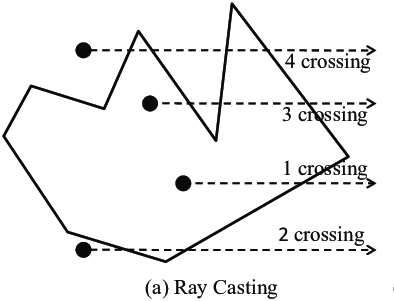
\includegraphics[width=0.3\linewidth]{img/raycrossingalgo.png}
    \caption{\centering\textit{Ray Crossing Algorithm (zdroj: Yan 2012)}}
    \label{fig:raycrossing}
\end{figure}
\vspace{1.5cm}




Pokud je počet průsečíků lichý, bod se nachází uvnitř polygonu, pokud je sudý, bod se nachází vně polygonu.
\vspace{1.5cm}
\[
k(q, P) =
\begin{cases}
1, & q \in P, \\
0 \ \text{nebo} \ 2, & q \notin P.
\end{cases}
\]
\vspace{1.5cm}

\noindent Problémem pro tento algoritmus jsou speciální případy, kde se bod nachází na hraně polygonu či na jeho vrcholu. Pro ošetření těchto speciálních případů je nutné zavést druhou polopřímku, která leží v opačném směru. Dále se postupuje u obou polopřímek stejným způsobem a počítají se průsečíky s hranami polygonu. Pokud se počet průsečíků obou polopřímek nerovná, bod leží na hraně/vrcholu polygonu.

\newpage
\section {Winding Number Algorithm}
\vspace{5mm}
Tento algoritmus je založen na „ovíjení“ a sčítání úhlů, které svírají vrcholy polygonu k bodu \textit{q}. Výsledné číslo Winding Number $\Omega$ se poté dělí $2\pi$ a dává nám tedy údaj o počtu „ovinutí“ okolo bodu \textit{q}. Pro to, zda se úhly přičtou či odečtou k výslednému Winding Number $\Omega$, se využívá koncept rozdělení na dvě poloroviny a výpočtu determinantu \textit{t} dvou vektorů: směrového vektoru hrany polygonu $\vec{p}$ a vektoru $\vec{v}$ směřujícího z počátečního vrcholu hrany k bodu \textit{q}:
\vspace{1cm}
\[
\begin{aligned}
\vec{p} &= (x_{i+1} - x_i, y_{i+1} - y_i) \\
\vec{v} &= (x_q - x_i, y_q - y_i)
\end{aligned}
\]
\vspace{1cm}

\noindent Po výpočtu vektorů se spočítá jejich vektorový součin (determinant):
\vspace{1cm}

\[
t = \det \begin{pmatrix} p_x & p_y \\ v_x & v_y \end{pmatrix}
\]
\vspace{1cm}

\noindent Na základě výsledného determinantu se určí v jaké polorovině bod q leží a zda se úhel bude přičítat či odčítat od výsledného Winding Number. Pokud \textit{t} > 0, bod \textit{q} leží v levé polorovině a úhel se přičítá, když \textit{t} < 0, bod \textit{q} náleží právé polorovině a úhel se odečítá, v případě \textit{t} = 0, bod \textit{q} leží na přímce a poté platí následující:
\vspace{1cm}
\[
\exists \omega(p_i, q, p_{i+1}) = \pi
\]
\vspace{1cm}

\noindent Pro výsledné Winding Number platí následující vztah:
\vspace{1cm}

\[
\Omega(q, P) = \frac{1}{2\pi} \sum_{i=1}^{n} \omega(p_i, q, p_{i+1})
\]
\vspace{1cm}




\newpage
\section {Aplikace}
\vspace{5mm}
Aplikace se otevře spuštěním skriptu MainForm.py a otevře se interaktivní okno, ve kterém lze zakreslit bod a polygon. Nad lištou tlačítek se nachází nabídka tří možností: \textit {File}, \textit {Input} a \textit {Analyze}. Po rozkliknutí záložky \textit {File} se nabídne možnost vložení vlastní polygonové vrstvy z počítače uživatele. Tlačítko \textit {Input} slouží pro přepnutí mezi zakreslením bodu nebo polygonu. Záložka \textit {Analyze}  nabízí dvě metody pro vyhledání polohy bodu. Dále je okno doplněno o záložku \textit {Open}, které nabízí možnost vložení souboru ve formátu shapefile, nad kterým lze provést zpracované algortimy: \textit {Ray Crossing Algorithm} a \textit {Winding Number Algorithm}. Pod hlavní lištou jsou v nabídce tlačítka pro provedení analýzy zpracovaných alogritmů, tlačítko na změnu zakreslení bodu a polygonu a tlačítko pro smazání aktuální vrstvy polygonu a bodu.
\vspace{3mm}

\noindent V případě vložené vlastní polygonové vrstvy se velikost zobrazované vrstvy přizpůsobí otevřenému oknu aplikace. Po zakreslení bodu, lze provést obě zmiňované metody vyhledávání bodu. 
\vspace{3mm}

\noindent Po spuštění analýzy pomocí libovolné metody se zobrazí informační okno, které uživateli sdělí zda se bod nachází uvnitř, vně či na hranici polygonu. Toto okno lze poté zavřít a bod překreslit na jiné místo a analyzovat jeho polohu znovu. Tlačítkem \textit {OK} se informační okno zavře a pomocí tlačítka \textit {Clear data} se smaže aktuální zakreslený polygon nebo vložená polygonová vrstva.
\vspace{1cm}

\begin{figure}[h!]
    \centering
    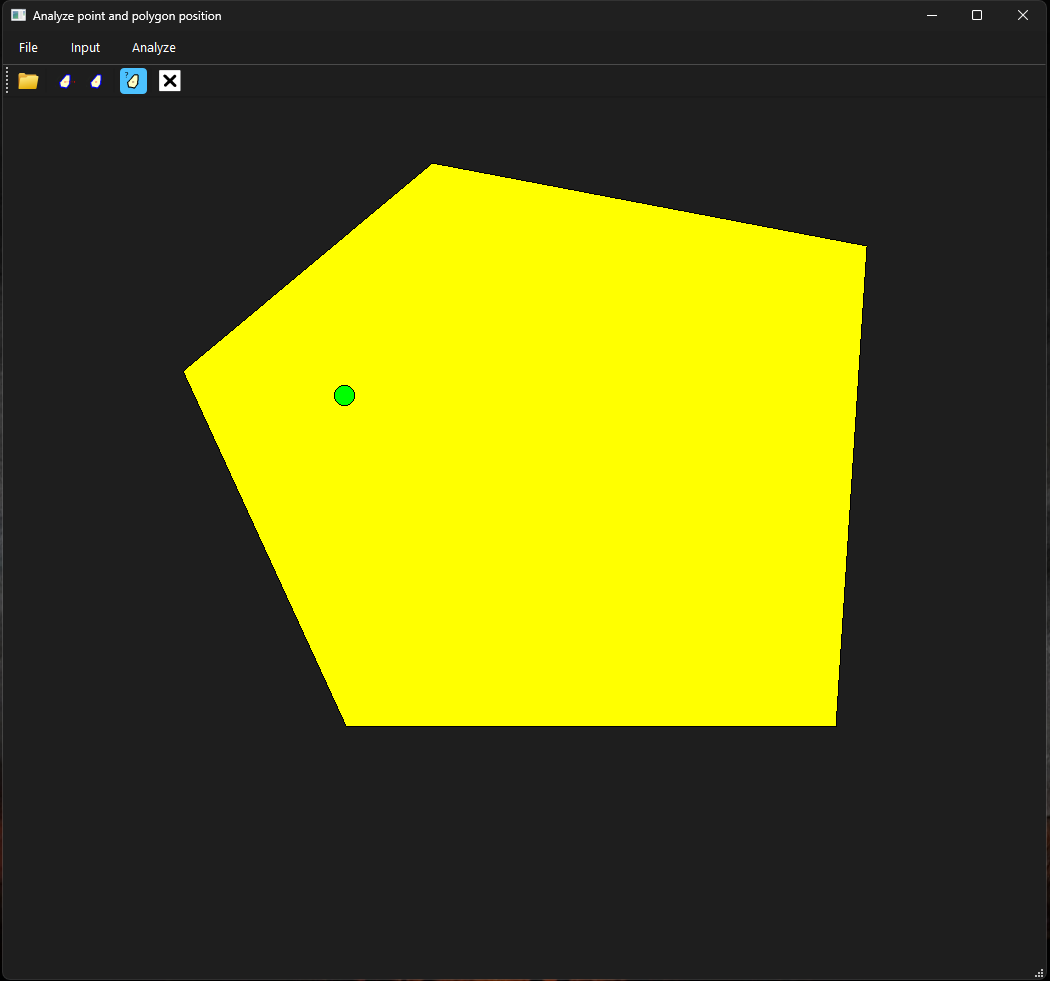
\includegraphics[width=0.5\linewidth]{img/aplikace_okno.png}
    \caption{\centering\textit{Uživatelské prostředí aplikace}}
    \label{fig:placeholder}
\end{figure}


\newpage
\section {Dokumentace}
\vspace{5mm}
Úloha byla vypracována v softwaru Visual Studio Code v jazyce Python a obsahuje 3 soubory se skripty, které na sebe odkazují (algorithms.py, draw.py, MainForm.py). Pro zapisování skriptů byl použit formát CamelCase. 
\vspace{5mm}
\subsection*{algorithms.py}
\vspace{3mm}
V tomto souboru byly uloženy následující funkce:
\vspace{3mm}

\begin{itemize}
    \item \textbf{def pointOnVertex} - Funkce zjišťuje zda se bod q nachází na vrcholu polygonu P, pokud se souřadnice x a y shodují, bod leží na vrcholu polygonu.
    \item \textbf{def rayCrossing} - Funkce analyzuje polohu bodu vůči polygonu metodou Ray Crossing Algorithm. Funkce prochází pomocí cyklu for každý vrchol polygonu. V případě že se bod nachází vně polygonu algoritmus vrací hodnotu 0, pokud se bod nachází uvnitř polygonu algoritmus vrací hodnotu 1 a v případě, že bod leží na vrcholu či hraně polygonu vrací algoritmus hodnotu -1. 
    \item \textbf{def calculateAngle} - Tato funkce vypočítává velikost vnitřního úhlu mezi vektorem v1 a v2. Pro výpočet úhlu nejprve vypočítá vektory vycházející z bodu q do bodů P1 a P2. V dalším kroce spočítá jejich délku a poté spočítá úhel mezi vektory. 
    \item \textbf{def getPointLocation} - Funkce analyzuje polohu bodu a přímky definovanou body P1 a P2 výpočtem determinantu. Pokud det = 0, bod leží na přímce, v případě když det > 0, bod leží vlevo od přímky, v případě det < 0, bod leží vpravo od přímky.
    \item \textbf{def windingNumber} - Funkce analyzuje polohu bodu vůči polygonu metodou Winding Number Algorithm. Pomocí cyklu while prochází všechny přímky (spojnice mezi vrcholy polygonu). V případě že se bod nachází uvnitř polygonu vrací hodnotu 1, pokud se bod nachází vně polygonu vrací hodnotu 0 a pokud se bod nachází na vrcholu či hraně vrací hodnotu -1. 
    \item \textbf{def inMinMaxBox} - Funkce kontroluje zda se bod nachází v min-max boxu polygonu. V případě, že se bod nenachazí v min-max boxu daného polygonu nemusí se provádět výpočet algoritmu pro vyhodnocení polohy bodu vůči polygonu, protože s jistotou v daném polygonu neleží. 
\end{itemize}

\vspace{5mm}
\subsection*{draw.py}
\vspace{3mm}
V tomto souboru byly uloženy následující funkce:
\vspace{3mm}

\begin{itemize}
    \item \textbf{def mousePressEvent} - Funkce určuje souřadnice zakreslení bodu nebo vrcholu polygonu, na základě kliknutí do plátna v aplikaci.
    \item \textbf{def changeStatus} - Funkce přepíná mezi kreslením polygonu nebo bodu.
    \item \textbf{def paintEvent} - Funkce vykreslí polygon, polygonovou vrstvu či bod do plátna. 
    \item \textbf{def clearData} - Funkce vymaže vykreslená data.
    \item \textbf{def getQ} - Funkce vrací analyzovaný bod.
    \item \textbf{def getPol} - Funkce vrací vykreslený polygon.
    \item \textbf{def getPolygons} - Funkce vrací polygony jako seznam, pokud se jedná o vrstvu s více polygony.
    \item \textbf{def setHighlightedPolygons} - Funkce nahradí seznam zvýrazněných polygonů na nový seznam indexů.
    \item \textbf{def paintRes} - Funkce přidá vybraný polygon do seznamu zvýrazněných polygonů.
    \item \textbf{def clearRes} - Funkce vymaže vykreslený polygon nebo vykreslenou polygonovou vrstvu a bod.
    \item \textbf{def openFile} - Funkce otevře systémové okno, ve kterém je možnost nahrání vlastní polygonové vrstvy ve formátu *.shp.
    \item \textbf{def loadSHP} - Funkce vykreslí zvolenou polygonovou vrstvu formátu *.shp do aplikace a polygony zařadí do seznamu. Funkce zajišťuje zpracování vstupní geometrie a upraví ji na souřadnice dle velikosti plátna aplikace. 
\end{itemize}

\vspace{5mm}
\subsection*{MainForm.py}
\vspace{3mm}
V tomto souboru byly uloženy následující funkce:
\vspace{3mm}

\begin{itemize}
    \item \textbf{def openFileClick} - Funkce zavolá funkci openFile.
    \item \textbf{def changeStatusClick} - Funkce zavolá funkci changeStatus.
    \item \textbf{def clearClick} - Funkce zavolá funkci clearData.
    \item \textbf{def getRes} - Funkce zavolá funkci getQ a skript algorithms.py. Funkce zajišťuje průběh algoritmů nad analyzovaným bodem a vstupním polygonem nebo vstupní polygonovou vrstvou. Nejdříve proběhne funkce inMinMaxBox a v případě, že bod náleží min-max boxu polygonu postupuje dále a na základě zvoleného algoritmu analyzuje polohu bodu k polygonu. 
    \item \textbf{def analyzePointAndPositionClick} - zavolá funkci getRes pro zvolený algoritmus Ray Crossing.
    \item \textbf{def analyzePointAndPositionWNClick} - zavolá funkci getRes pro zvolený algoritmus Winding Number.
\end{itemize}


\newpage
\section*{Seznam literatury}
\vspace{5mm}
BAYER, Tomáš. {\textit Algoritmy v digitální kartografii}. Praha: Karolinum, 2008. ISBN 978-80-246-1499-1.
\vspace{3mm}

\noindent BAYER, T. (2026): Point Location Problem. Prezentace pro přednášku předmětu Algoritmu počítačové kartografie, Katedra aplikované geoinformatiky  a kartografie, Přírodovědecká a fakulta UK [cit. 22. 3. 2026].
\vspace{3mm}

\noindent AN, D., ZHAO, Z., NG, W. K. (2012): Monochromatic and Bichromatic Reverse Nearest Neighbor Queries on Land Surfaces. 10.1145/2396761.2396880.

\end{document}


